\chapter{Our Proposal: Framework Design}

We propose two major future versions of idock, plus a few other methodological enhancements.

\section{idock 2.0: GPU Acceleration}

\subsection{Motivation}

Even though idock 1.6 outperformed AutoDock Vina \citep{595} by at least 8.69 times and at most 37.51 times in terms of docking speed and was capable of docking 16 ligands per minute on a high performance machine, it is estimated to require about 312 days, i.e. nearly a year, to dock the complete 7,220,835 drug-like ligands from ZINC against a certain protein, not to mention multiple proteins. Virtual screening remains a time-consuming practice. Faster implementations are highly desired.

We used AMD CodeAnalyst Performance Analyzer v3.6 to detect program hotspots and observe thread behaviors. Figure \ref{idock:ThreadProfile} shows the thread profile of idock. Thread 1060 was the main thread, while the other four were workers threads spawned by the main thread and maintained by our novel thread pool. During program startup, the main thread parsed command line arguments, initialized necessary variables, parsed receptor file, and created a thread pool to precalculate the scoring function in parallel. Afterwards, it entered a loop, docking ligands one by one. The four workers threads actually carried out the creation of grid maps as well as running Monte Carlo tasks in parallel, fully occupying all the four CPU cores. Upon completion of docking a ligand, program control was returned to the main thread to write conformations to file and read the next ligand from file. From the figure, it can be concluded that the worker threads acquire most of the CPU computing resources and the precalculation of grid maps and the execution of Monte Carlo tasks constitute the program hotspots, albeit the CPU-intensive Monte Carlo tasks and the I/O-intensive file reading/writing can be possibly pipelined according to our in-house trial.

\begin{figure}
\centering
\includegraphics[width=\textwidth]{idock/ThreadProfile.png}
\caption{idock thread profile.}
\label{idock:ThreadProfile}
\end{figure}

We propose idock 2.0, incorporating GPU acceleration with both CUDA and OpenCL, harnessing the tremendous computational power and memory bandwidth offered by modern GPUs nowadays. In \citeyear{1138} we developed a fast CUDA implementation of agrep algorithm for approximate nucleotide sequence matching \citep{1138}, demonstrating our expertise in CUDA programming. Meanwhile, we are eagerly learning OpenCL. We will first work on a CUDA version, followed by an OpenCL version.

\subsection{Strategies}

Performance optimization revolves around three basic strategies: 1) maximizing parallel execution, 2) maximizing memory bandwidth, and 3) maximizing instruction throughput.

Maximizing parallel execution can be achieved by exposing as much data parallelism as possible and mapping the parallelism to the hardware as efficiently as possible. In dock, we have parallelized both the precalculation of grid maps and the Monte Carlo global optimization using our novel thread pool in order to thoroughly utilize multicore CPU. We plan to port these two most time-consuming parts to the GPU, map Monte Carlo tasks directly to CUDA threads, and use NVIDIA's occupancy calculator to carefully choose the execution configuration of each kernel launch in order to maintain a high GPU utilization. Several technical difficulties exist. One difficulty is the lack of sufficient capacity of GDDR5 memory, which is merely 2GB along with a GeForce GTX 680. This restriction voids the precalculation of grid maps at a fine granularity like 0.08\AA, leading to reduced approximation accuracy and possibly a high false negative rate. Another difficulty is the efficient generation of pseudo random numbers. Although there are official libraries and third-party libraries to facilitate this purpose, it is hard to determine the number of random numbers in need in advance because the Monte Carlo algorithm is stochastic \textit{per se}.

Maximizing memory bandwidth can be achieved by minimizing data transfers between the CPU and the GPU and optimizing the access patterns to global memory and shared memory on the GPU. Since CPU-to-GPU and GPU-to-CPU data transfers have much lower bandwidth than internal GPU data transfers, we plan to accommodate as much data as possible into the GPU global memory. In idock 2.0, constant data such as structure of receptor, definition of search space, precalculation of scoring function, and configurations for the BFGS Quasi-Newton local optimizer will reside in constant cache, while grid maps, due to its huge size, will reside in global memory, and temporary variables will reside in per-thread registers.

Maximizing global memory bandwidth is of crucial importance, and its bandwidth depends largely on its access pattern. Figure \ref{GPU:AlignedSequentialGlobalMemoryAccess} shows an example of aligned and sequential global memory access and corresponding memory transactions based on compute capability. In this case, 32 threads of a warp access adjacent 4-byte words such as adjacent single precision float values or 32-bit integer values. In other words, the \textit{k}th thread accesses the \textit{k}th 4-byte word in a 128B L1 cache line, a single coalesced transaction alone will service that memory access. In idock 2.0, we will adopt this kind of aligned and sequential access pattern and re-organize array of structures into structure of arrays, e.g.  [ \{ x1, y1, z1 \}, \{ x2, y2, z2 \} ] into \{ [ x1, x2 ], [ y1, y2 ], [ z1, z2 ] \}. Such a restructuring requires rewriting almost all the relevant mathematical data structures and functions in use in idock. So far we have stepped towards this direction a little bit, finishing rewriting the template class of quaternion from the BOOST C++ library into our own lightweight version to represent the orientation of a conformation.

\begin{figure}
\centering
\includegraphics[width=\linewidth]{GPU/AlignedSequentialGlobalMemoryAccess.png}
\caption{Aligned and sequential global memory accesses by a warp, 4-byte word per thread, and associated memory transactions based on compute capability. Source: NVIDIA.}
\label{GPU:AlignedSequentialGlobalMemoryAccess}
\end{figure}

A GK104 SMX has 64KB of on-chip memory that can be configured as 48KB of shared memory with 16KB of L1 cache, or as 16KB of shared memory with 48KB of L1 cache. Since threads within a thread block run their Monte Carlo tasks independently and seldom communicate with one another, we decide to allocate 48KB of the 64KB on-chip memory to L1 cache.

Maximizing instruction throughput can be achieved by using single precision floating point instead of double precision and using intrinsics instead of regular functions. This strategy suggests trading precision for speed as long as the final result is not affected. Since most contemporary GPU chips supply with an astonishingly high throughput for single precision operations at TFLOP level but a relatively low throughput for double precision operations, we prefer the former. In order to make sure the precision loss must not affect the end result too much, we did an in-house trial, demoting double to float in idock, only to find that the predicted conformation and free energy were exactly identical as in the case of double precision given the same random seed for initializing the pseudo random number generator. This experiment concluded idock to be insensitive to precision switch and it is thus safe to utilize single precision operations as well as native intrinsics in idock 2.0.

\subsection{Future Work}

By then with idock 2.0 at hand, we shall be able to do two things that are not possible at present. One one hand, we shall fine tune the parameters of our BFGS local optimizer in order to increase the redocking success rate. Those parameters include the early stopping criterion, the step size in line search, the apprximation of inverse Hessian matrix, and so on. On the other hand, we shall perform proteomic-scale docking for the entire solved proteins in PDB \citep{540,537} and warehouse the huge results into a public database. We believe the community will definitely benefit from such a database with pre-docked information instantly available.

\section{idock 3.0: \textit{De Novo} Ligand Design}

\textit{De novo} ligand design and protein-ligand docking are closely related. Tiny fragments are combined in accordance to chemistry rules to synthesize larger ligands, which are then docked to a receptor to evaluate their fitness. The best ligands enter the next iteration to synthesize other ligands, which are again evaluated by docking, until promising ligands are discovered. AutoGrow \citep{466}, released in \citeyear{466}, is a representative \textit{de novo} ligand design tool that makes use of genetic algorithm and AutoDock Vina \citep{595} to automate this recursive synthesis/docking procedure.

In 2011, inspired by AutoGrow, we developed SmartGrow, addressing several problems that AutoGrow suffers from. SmartGrow not only inherited the selection, mutation and crossover operators from AutoGrow, but also invented our novel merge and split operators. It implemented Lipinski's \textit{Rule of Five} \citep{168} to ensure drug likeness. Its robust parser correctly processed two-letter chemical elements like Cl (chlorine) and Br (bromine), and meanwhile added additional support for P (phosphorus), a common chemical element found in many drugs. Results showed that SmartGrow displayed comparable performance in terms of predicted free energy and meanwhile outperformed AutoGrow by 30\% in terms of execution time on average across 18 test cases. Besides, ligands generated by SmartGrow resulted in 100g/mol lower molecular weights than AutoGrow and never exceeded 500g/mol so that they can be absorbed by human body.

However, we wrote SmartGrow in a hurry and did not follow a formal software engineering approach. Later on when we conducted a benchmark on SmartGrow, we discovered a great many of exceptional bugs that were rather hard to track due to the messy code structure and lack of comments. Regretfully, we decided to abandon our buggy SmartGrow.

\subsection{Methods and Novel Operators}

We then developed igrow as a successor of SmartGrow. Instead of porting existing code from SmartGrow and fixing bugs line by line, we rewrote igrow from scratch in a systematic manner. We borrowed several great ideas from idock, and deliberately designed igrow in the way that the output of idock directly feeds igrow as its input. Figure \ref{igrow:Flowchart} shows the flowchart of our current implementation of igrow. During initialization, igrow parses the initial elite ligands predicted by idock in a previous run, and scans a user-specified folder for fragments. Likewise in idock, igrow also creates a novel thread pool in order to parallelize the mutation and crossover operators and reuse threads throughout the entire synthesis procedure. Then igrow enters a loop, and utilizes genetic algorithm to iteratively synthesize novel ligands in parallel by either mutation or crossover, and invoke idock externally to predict free energy and select elite ligands by sorting the predicted free energy asendingly. So far we have completed the program, and are now fixing bugs and evaluating it.

\begin{figure}
\centering
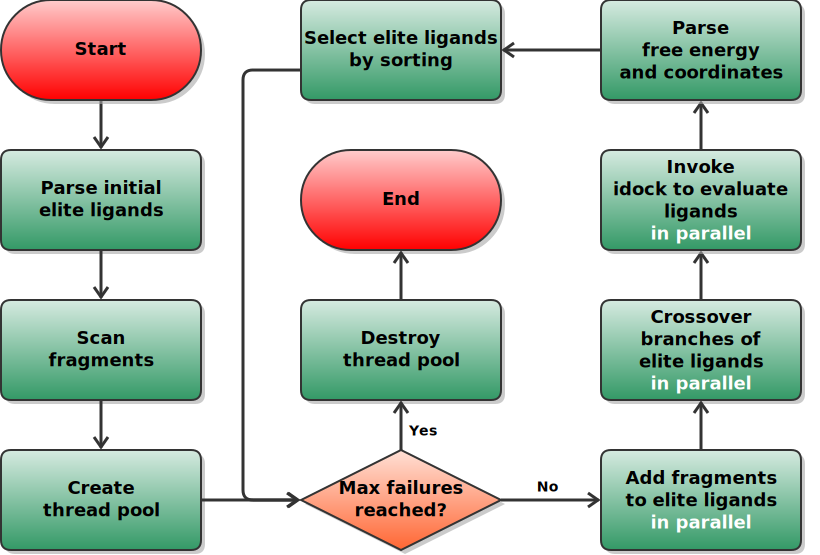
\includegraphics[width=\textwidth]{igrow/Flowchart.pdf}
\caption{igrow flowchart.}
\label{igrow:Flowchart}
\end{figure}

Figure \ref{igrow:Addition} illustrates the addition operator in igrow. An elite ligand and a fragment are randomly selected and merged by removing a hydrogen atom from both sides and forming a new rotatable bond to connect both sides, thereby constructing an elite ligand. The addition operator may produce novel ligands that display a higher binding affinity but may also suffer from a larger molecular weight. Figure \ref{igrow:AdditionComplex} draws the three elitsts in complex with their target protein. Due to the presence of additional fragments, the elite ligands may occupy significantly different binding conformations.

\begin{figure}
\centering
\includegraphics[width=\textwidth]{igrow/Addition.png}
\caption{igrow addition operator.}
\label{igrow:Addition}
\end{figure}

\begin{figure}
\centering
\includegraphics[width=\textwidth]{igrow/AdditionComplex.png}
\caption{Synthesized elitists by addition in complex with their target protein.}
\label{igrow:AdditionComplex}
\end{figure}

Figure \ref{igrow:Subtraction} illustrates the subtraction operator in igrow. An elite ligand and one of its rotatable bonds are randomly selected. The ligand is split into two by breaking the rotatable bond and substituting a hydrogen, thereby constructing a smaller ligand. The subtraction operator may produce novel ligands that display a lower binding affinity but may also benefit from a smaller molecular weight.

\begin{figure}
\centering
\includegraphics[width=\textwidth]{igrow/Subtraction.png}
\caption{igrow subtraction operator.}
\label{igrow:Subtraction}
\end{figure}

Figure \ref{igrow:Crossover} illustrates the crossover operator in igrow. Two elite ligands are randomly selected and parts of them are exchanged, thereby constructing an elite ligand. The crossover operator may produce novel ligands that display either a higher binding affinity or a lower binding affinity. Figure \ref{igrow:CrossoverComplex} draws the three elitsts in complex with their target protein. Due to the exchange of molecular moieties, the elite ligands may occupy significantly different binding conformations.

\begin{figure}
\centering
\includegraphics[width=\textwidth]{igrow/Crossover.png}
\caption{igrow crossover operator.}
\label{igrow:Crossover}
\end{figure}

\begin{figure}
\centering
\includegraphics[width=\textwidth]{igrow/CrossoverComplex.png}
\caption{Synthesized elitists by crossover in complex with their target protein.}
\label{igrow:CrossoverComplex}
\end{figure}

\subsection{Discussion}

Compared to AutoGrow and SmartGrow, our igrow features a plenty of advantageous innovations. From the perspective of input and output, igrow supports direct PDBQT manipulation, i.e. it digests ligands and fragments in PDBQT format and outputs ligands also in PDBQT format, saving the effort of frequently calling external python script for format conversion. igrow utilizes flyweight programming pattern to cache fragments and dynamic pointer vector to cache and sort ligands. From the perspective of CPU and memory utilization, igrow inherits from idock the highly efficient thread pool to parallelize the two genetic operators and maintain a high CPU utilization. igrow estimates the capacity of every vector structure and intensively utilizes right value reference, a new feature in the C++11 standard, to avoid frequent memory reallocation. From the perspective of functional improvements, in addition, igrow supports halogen replacement as a new type of synthesis in addition to hydrogen replacement, in subtraction, igrow supports spliting a ligand into two by breaking a rotatable bond and substituting a hydrogen, and in crossover, igrow supports branch replacement, and in selection, igrow refreshes ligands with docked coordinates, potentially enabling partial docking as detailed below. igrow traces the sources of synthesized ligands and outputs statistics in CSV format for users to easily analyze how new ligands are synthesized from initial elite ligands and fragments (Figure \ref{igrow:SyntheticTraceability}). igrow allows users to specify ranges of several chemical properties, including molecular weight, number of atoms, number of heavy atoms, number of rotatable bonds, number of hydrogen bond donors and number of hydrogen bond acceptors, as validators for newly synthesized ligands. igrow is designed in a flexible way that it reserves room for adaptation to new molecular constraints. Instead of simply depending on the number of generations as a stopping criterion, igrow allows users to specify the number of validation failures as a more reasonable stopping criterion.

\begin{figure}
\centering
\includegraphics[width=\textwidth]{igrow/SyntheticTraceability.png}
\caption{igrow synthetic traceability.}
\label{igrow:SyntheticTraceability}
\end{figure}

Clearly, there are two major problems with our current design. Problem one is the chemical infeasibility of ligands synthesized. This is a functional problem. Problem two is the high cost of invoking external idock in every generation. This is a computational problem.

Functionally speaking, ligands synthesized by our mutation and crossover operators, albeit chemically valid, might not be chemically synthesizable, simply because the two operators are somewhat arbitrary and do not conform to any known or general chemical reactions. In other words, that we can computationally synthesize novel ligands does not imply we can chemically synthesize them in reality. We may produce very fancy ligands at will, but all are just in computer simulation.

Computationally speaking, igrow relies on idock as its external docking engine and thus has to invoke idock every generation after synthesizing new ligands, repeatedly reading identical receptor and creating identical grid maps. Such duplications prolong program execution time quite a bit as the number of generations increases in genetic algorithm.

We propose idock 3.0 to address the above two problems. On one hand, inspired by AutoClickChem \citep{1051}, we plan to incorporate click chemistry into igrow to make sure every step of synthesis does follow some kind of well-known chemical reaction. On the other hand, we plan to integrate igrow into idock. In addition to receptor and grid map caching, another advantage of integration is the capability of partial docking, which refers to holding the main body of a ligand rigid while merely rotating newly added fragments. By cutting off the positional and orientational degrees of freedom, obviously partial docking can dramatically reduce search space dimensionality and therefore dramatically speed up the selection operator, which is the bottleneck of igrow.

\subsection{Software Availability}

As for software availability, igrow is free and open source under Apache License 2.0. It is written in C++ and available at https://github.com/HongjianLi/igrow. Precompiled executables for 32-bit and 64-bit Linux, Windows, Mac OS X, FreeBSD and Solaris are provided. Use cases and API documentations are also provided.

\section{iview: HTML5 Visualizer}

Currently the output of idock on istar include docked conformations in PDBQT format. Users have to download them and visualize them using their favorite molecular visualizer, such as PyMOL \citep{1221}, Chimera \citep{1219}, VMD \citep{1220}, AutoDockTools4 \citep{596}, ViewDock TDW \citep{559}, PoseView \citep{748} and LigPlot+ \citep{951}.

Inspired by iCanPlot, a visualizer of high-throughput omics data using interactive HTML5 canvas plotting \citep{1028}, we propose iview, an interactive HTML5 visualizer of protein-ligand complex (Figure \ref{istar:iview}). Users shall be able to view the protein-ligand docking results directly on istar. Typical functionalities include zooming, dragging, and plotting hydrogen bonds.

\begin{figure}
\centering
\includegraphics[width=\linewidth]{istar/iview.png}
\caption{iview is an interactive HTML5 visualizer of protein-ligand complex.}
\label{istar:iview}
\end{figure}

\section{Local Search Pruning}

Recall that idock uses Monte Carlo algorithm for global optimization and BFGS (Broyden-Fletcher-Goldfarb-Shanno) Quasi-Newton method \cite{786} for local optimization. It is possible to prune hopeless local search heuristically because a local minimum must be a stationary point with zero derivative in a continuous function, which is the case of the scoring function used in idock, according to Fermat’s theorem.

Figure \ref{idock:FunctionLandscape}, reprinted from \citep{1193}, shows a continuous function in 1D space for illustration purpose. Points A, B, and D are with negative derivatives while C is with a positive derivative. According to the intermediate value theorem, there must be a stationary point with zero derivative between A and C, but not guaranteed between A and B.

\begin{figure}
\centering
\includegraphics[width=\textwidth]{idock/FunctionLandscape.png}
\caption{Illustration of a 1D function landscape. Points A, B, and D are with negative derivative and point C is with positive derivative. Figure reprinted from \citep{1193}}
\label{idock:FunctionLandscape}
\end{figure}

We propose a heuristic to check whether a Monte Carlo starting point should undergo local search by testing it against the recent history of visited points. If there is a neighboring point with entirely opposite signs of derivatives in every dimension, the starting point should undergo local search, otherwise another random starting point should be picked, pruning a hopeless local search. Utilizing this heuristic, QuickVina \citep{1193} was reported to achieve an average speed-up of 8.34 times compared to AutoDock Vina \citep{595}.

Neverthelss, this heuristic might cause false negatives. Two points with derivatives of the same sign do not always imply there are no stationary points in between. We shall work on this issue by plotting and throughly analyzing the landscape of the scoring function.

\section{Dual-Ligand Docking}

We propose dual ligand docking, which refers to docking two ligands simultaneously inside one single large binding site, in order to achieve synergistic effect of two inhibitors. This feature is especially handy when the binding site is so large that it can accommodate more than one ligand. An example is the tail-loop binding site of influenza A nucleoprotein (Figure \ref{idock:2IQHDualLigands}).

\begin{figure}
\centering
\includegraphics[width=\textwidth]{idock/2IQHDualLigands.png}
\caption{Dual ligand docking.}
\label{idock:2IQHDualLigands}
\end{figure}

The existing scoring function shall be revised to properly merge individual scores into an overall one. The existing search algorithm shall also be revised to avoid possible steric clashes between the two ligands.

\section{Ligand Clustering}

On our istar platform, due to as many as 12 millions to dock, we propose hierarchical ligand clustering and thus estimating similar ligands as a whole rather than individually in order to avoid unnecessary docking and thus accelerate the entire docking procedure. Figure \ref{istar:LigandClustering} plots six ligands with the same skeleton.

\begin{figure}
\centering
\includegraphics[width=\textwidth]{istar/LigandClustering.png}
\caption{Ligands sharing an identical skeleton can be clustered hierarchically.}
\label{istar:LigandClustering}
\end{figure}

Clustering requires a measurement of similarity. Indeed, there are multiple ways to estimate the similarity between any two ligands. Most methods tend to account for molecular topology. Related work includes SIML \citep{726} and Tanimoto matrix calculation \citep{881} for chemical similarity calculation, PAPER \citep{491} for molecular shape comparison and CAMPAIGN \citep{932} for data clustering.

We propose our own hierarhical ligand clustering method, and apply it to our large dataset. Probably we shall make use of GPU acceleration for this intensive clustering task.

\section{ADMET Property Prediction}

It was estimated that 40\% to 60\% of new chemical entity (NCE) failures can be attributed to poor ADMET (absorption, distribution, metabolism, excretion, and toxicity) profiles. Accurately predicting ADMET properties is getting more and more attention nowadays.

PKKB (PharmacoKinetics Knowledge Base) \citep{1133} provides the most extensive collection of freely available data for ADMET properties up to date. PKKB integrates 31,412 experimental or predicted values for 1,685 drug and drug-like molecules from published literature with available experimental ADMET properties including partition coefficient (logP), solubility (logS), intestinal absorption, Caco-2 permeability, human bioavailability, plasma protein binding, volume of distribution, distribution of blood, half-time, excretion, urinary excretion, clearance, toxicity, etc. (Table \ref{PKKB:Properties})

\begin{table}
\centering
\begin{tabular*}
{\linewidth}
{@{\extracolsep{\fill}}rlr}
\toprule
No. & Property & Measurements \\
\midrule
\multicolumn{3}{l}{\textbf{Molecular properties}}\\
1 & Molecular weight & 1,684 \\
2 & logP (experiment) & 1,019 \\
3 & logP (predicted, AB/logP v2.0) & 1,625 \\
4 & Pka & 638 \\
5 & logD (pH=7,predicted) & 1,625 \\
6 & Solubility (experiment) & 800 \\
7 & logS (predicted, ACD/Labs)(pH=7) & 1,614 \\
8 & logSw (predicted, AB/LogSw 2.0) & 1,625 \\
9 & Sw (mg/ml) (predicted, ACD/Labs) & 1,613 \\
10 & Sw (predicted) & 1,625 \\
11 & No. of hbond donors & 1,625 \\
12 & No. of hbond acceptors & 1,625 \\
13 & No. of rotatable bonds & 1,625 \\
14 & TPSA & 1,625 \\
\noalign{\smallskip\smallskip}
\multicolumn{3}{l}{\textbf{Pharmacology}}\\
15 & Status & 1,372 \\
16 & Administration & 501 \\
17 & Pharmacology & 1,543 \\
\noalign{\smallskip\smallskip}
\multicolumn{3}{l}{\textbf{Absorption}}\\
18 & Intestinal absorption & 679 \\
19 & Absorption (description) & 699 \\
20 & Caco-2 & 64 \\
21 & Human bioavailability & 992 \\
\noalign{\smallskip\smallskip}
\multicolumn{3}{l}{\textbf{Distribution}}\\
22 & Plasma protein binding & 1058 \\
23 & Volume of distribution(Vd) & 646 \\
24 & D-blood & 66 \\
\noalign{\smallskip\smallskip}
\multicolumn{3}{l}{\textbf{Metabolism}}\\
25 & Metabolism & 1,111 \\
26 & Half-time & 1,116 \\
\noalign{\smallskip\smallskip}
\multicolumn{3}{l}{\textbf{Excretion}}\\
27 & Excretion & 855 \\
28 & Urinary excretion & 281 \\
29 & Clearance & 410 \\
\noalign{\smallskip\smallskip}
\multicolumn{3}{l}{\textbf{Toxicity}}\\
30 & Toxicity & 873 \\
31 & LD50 (rat) & 219 \\
32 & LD50 (mouse) & 243 \\
\bottomrule
\end{tabular*}
\caption{PKKB property measurements. Data obtained from PKKB web site.}
\label{PKKB:Properties}
\end{table}

Figure \ref{PKKB:Schema}, reprinted from \citep{1133}, shows the PKKB schema. Raw data from literature was first converted into proper formats and then integrated into a central ADMET database. A web site is provided for interactive search of ADMET properties given either structure or descriptive text of compounds of interest.

\begin{figure}
\centering
\includegraphics[width=\linewidth]{PKKB/Schema.jpg}
\caption{PKKB schema. Figure reprinted from \citep{1133}.}
\label{PKKB:Schema}
\end{figure}

Thanks to the availability of reliable experimental data and basic structural information from PKKB enables, \textit{in silico} ADMET modeling becomes viable. One can predict ADMET properties from chemical structures for a huge number of compounds without actually synthesizing or assaying them.

We propose to make use of advanced machine learning techniques to train a regression model (Figure \ref{PKKB:Regression}), be it linear or non-linear. Once the model is constructed, it is possible to predict ADMET properties of any given compounds. Coupled with conformations and free energy predicted by our tool idock, we can better evaluate a compound from a wide variety of perspectives, leading to a higher drug discovery success rate. Moreover, such a regression model can be integrated into igrow to guide ligand synthesis, which can then be further integrated into idock to guide ligand filtering and eventually into istar to compose a comprehensive framework for structure-based drug discovery.

\begin{figure}
\centering
\includegraphics[width=\linewidth]{PKKB/Regression.png}
\caption{Our proposed regression model for PKKB.}
\label{PKKB:Regression}
\end{figure}

\chapterend
